\documentclass[ngerman,aspectratio=169,10pt]{beamer}

\usetheme[progressbar=frametitle]{metropolis}
\usepackage{appendixnumberbeamer}

\graphicspath{{./graphics/}}

\usepackage{booktabs}
\usepackage{xspace}
\usepackage{amsmath}
\usepackage{amssymb}
\usepackage{amsthm}
\usepackage{xfrac}
\usepackage{listings}
\lstset{
	basicstyle=\ttfamily,
	showstringspaces=false,
	tabsize=4,
	upquote=true,
}

\title{LOUDS++}
% \subtitle{}
% \date{16. November 2020}
\author{Finn Stutzenstein, Levin Nemesch, Joshua Sangmeister}
\institute{Algorithm Engineering - Übung 2}
\titlegraphic{
    \hfill
\includegraphics[height=1.5cm]{unilogo.pdf}\\
    \hspace*{8.3cm} \textsc{AG Theoretische Informatik}
}

\begin{document}

\maketitle

\begin{frame}{Überblick}
    \begin{itemize}
        \item LOUDS: Level-Order Unary Degree Sequence
        \item \emph{succinct data structure}: $2n + o(n)$ Bits Speicherbedarf
        \item Geordneter Baum
        \item Unterstützt folgende Operationen in $\mathcal{O}(1)$:
        \begin{itemize}
            \item parent(x)
            \item first-child(x)/last-child(x)
            \item prev-sibling(x)/next-sibling(x)
            \item degree(x): Anzahl der Kinder von x
            \item childrank(x): Rang von x unter seinen Geschwistern
            \item child(x, i): i-tes Kind von x
        \end{itemize}
    	\item Quelle: "Engineering the LOUDS Succinct Tree Representation" von O'Neil Delpratt, Naila Rahman, and Rajeev Raman (\url{https://citeseerx.ist.psu.edu/viewdoc/download?doi=10.1.1.106.4250&rep=rep1&type=pdf})
    \end{itemize}
\end{frame}

\begin{frame}{Bitvektor}
    \begin{itemize}
        \item<1-> Bitfeld von $n$ Bits
        \item<1-> $\texttt{rank}_b(x)$ ($b\in\{0,1\}$): Anzahl der Vorkommnisse von $b$ bis $x$
        \item<1-> $\texttt{select}_b(x)$ ($b\in\{0,1\}$): Position des $x$-ten Vorkommens von $b$
        \item<1-> Z.B. von Kim Et Al.: Speicher $n+o(n)$ Bits und Laufzeiten in $\mathcal{O}(1)$
        \item<2-> Beispiel: \texttt{0011011100}
            \begin{itemize}
                \item $\texttt{rank}_1(7)=4$
                \item $\texttt{rank}_0(7)=3$
                \item $\texttt{select}_1(3)=6$
                \item $\texttt{select}_0(5)=10$
            \end{itemize}
    \end{itemize}
\end{frame}

\begin{frame}{LOUDS bit string (LBS)}
    \begin{itemize}
        \item Speichert unär Baumstruktur
        \item Jeder Knoten repräsentiert durch $1^d0$ Bitstring, $d$ entspricht Anzahl Kinder
        \item Nummerierung der Knoten ebenenweise (entspricht Breitensuche)
        \item Beginn markiert durch $10$
    \end{itemize}
\end{frame}

\begin{frame}{LOUDS}
    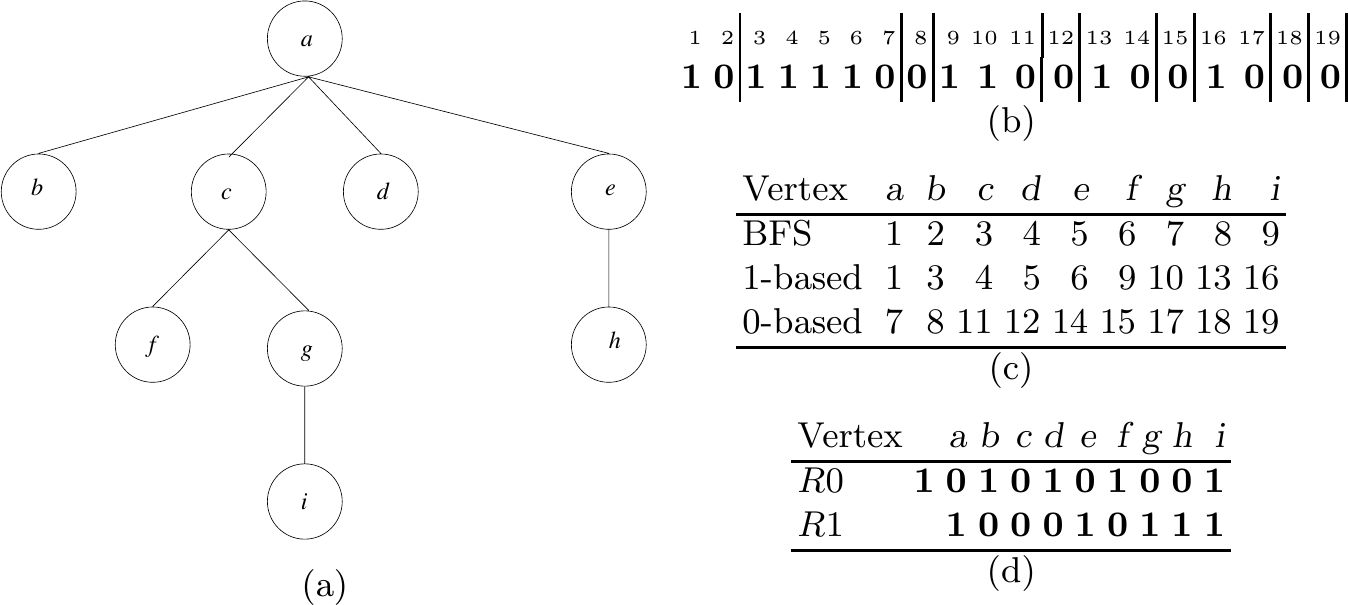
\includegraphics[width=1.0\textwidth]{LOUDS.jpg}
\end{frame}

\begin{frame}{Eigenschaften LBS}
    \begin{itemize}
        \item Besteht aus $n+1$ 0-en und $n$ 1-en
        \item $i$-ter Knoten:
        \item \textit{Ones-based numbering}
        \begin{itemize}
            \item $i$-te 1 in Kodierung des Elternknotens
            \item Knoten $i$ wird Zahl $x=\texttt{select}_1(i)\in\{1,\ldots,2n+1\}$ zugewiesen
            \item Knoten mit Zahl $x$: $i=\texttt{rank}_1(x)\in\{1,\ldots,n\}$
        \end{itemize}
        \item \textit{Zero-based numbering}: $i+1$-te 0: Ende der Kodierung des $i$-ten Knotens
        \begin{itemize}
            \item $i+1$-te 0: Ende der Kodierung des $i$-ten Knotens
            \item Mit $\texttt{select}_0$ und $\texttt{rank}_0$ kann analog zum Ones-based numbering eine Zahl zugeordnet werden
        \end{itemize}
    \end{itemize} 
\end{frame}

\begin{frame}{Beispiel: Operation $\texttt{parent}(x)$}
    \begin{center}
        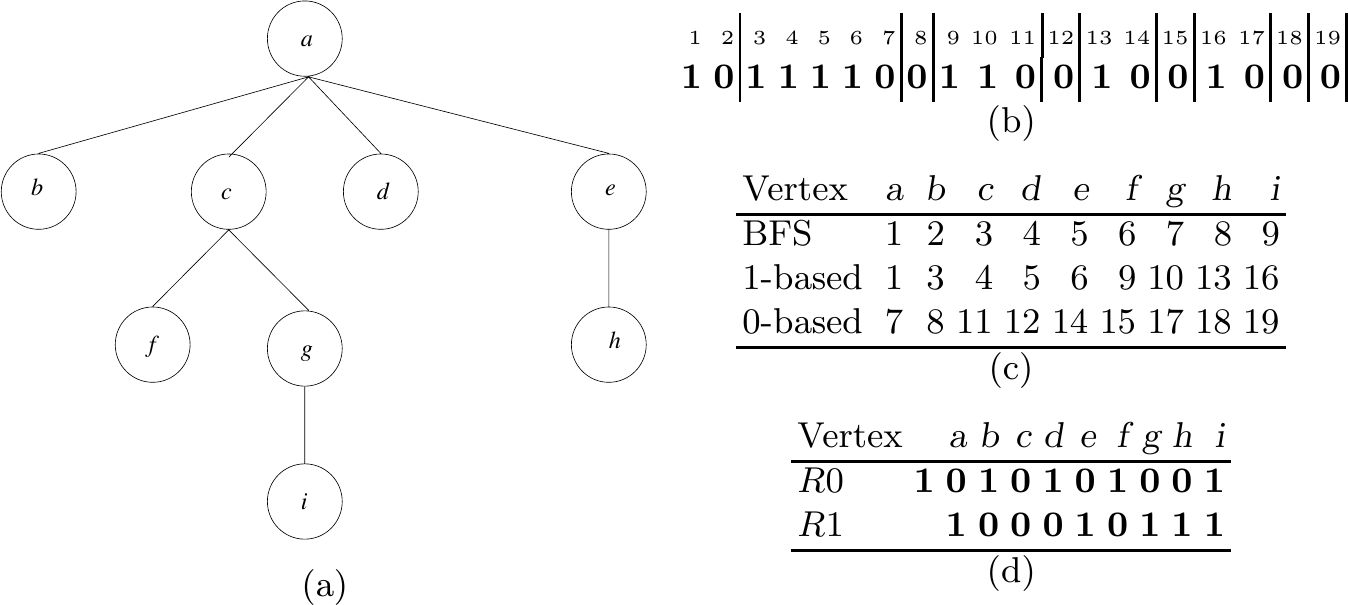
\includegraphics[width=0.7\textwidth]{LOUDS.jpg}
    \end{center}
    \begin{columns}
		\begin{column}{0.55\textwidth}
			\begin{itemize}
                \item \textit{Ones-based numbering:}\\ $x=\texttt{select}_1(\texttt{rank}_0(x))$
                \item \textit{Zero-based numbering:}\\ $\texttt{select}_0(\texttt{rank}_0(\texttt{select}_1(\texttt{rank}_0(x)-1)+1))$
            \end{itemize}
		\end{column}
		\begin{column}{0.45\textwidth}
		    \only<1>{
		        Beispiel \texttt{parent}(g) (Ones-based):\\
		        Knoten g (BFS 7) $\rightarrow$ $\texttt{select}_1(7)=10$\\
		        $\texttt{rank}_0(10)=3$\\
		        $\texttt{select}_1(3)=4$\\
		        $\texttt{rank}_1(4)=3$ $\rightarrow$ Knoten c (BFS 3)
		    }
		    \only<2>{
		        Beispiel \texttt{parent}(g) (Zero-based):\\
		        $\texttt{rank}_0(17)-1=8-1=7$\\
		        $\texttt{select}_1(7)+1=10+1=11$\\
		        $\texttt{rank}_0(11)=4$\\
		        $\texttt{select}_0(4)=11$\\
		    }
		\end{column}
	\end{columns}
\end{frame}

\begin{frame}[fragile]{Double-Numbering}
    \begin{itemize}
        \item $y=\texttt{select}_0(x)\implies \texttt{rank}_0(y)=x\wedge \texttt{rank}_1(y)=y-x$
        \item analog für $\texttt{select}_1$
        \pause
        \item Beispiel: \texttt{0011011100}
            \begin{itemize}
                \item $\texttt{select}_0(4)=9$
                \item $\rightarrow \texttt{rank}_0(9)=4$
                \item $\rightarrow \texttt{rank}_1(9)=9-4=5$
            \end{itemize}
        \pause
        \item Punkte können somit als Paar $\{x, y\}$ gespeichert werden
        \item Aufrufe der Form \texttt{rank(select($\dots$))} können durch einfache \texttt{select}s ersetzt werden
        \item Beispiel für \texttt{parent}:
    \end{itemize}
	\begin{lstlisting}[escapechar=|]
	parent({x, y}):
		rzerox = y - x
		newy = select|$_1$|(rzerox)
		newx = newy - rzerox
		return {newx, newy}
	\end{lstlisting}
\end{frame}

\begin{frame}{Partitioned Representation}
    \begin{center}
        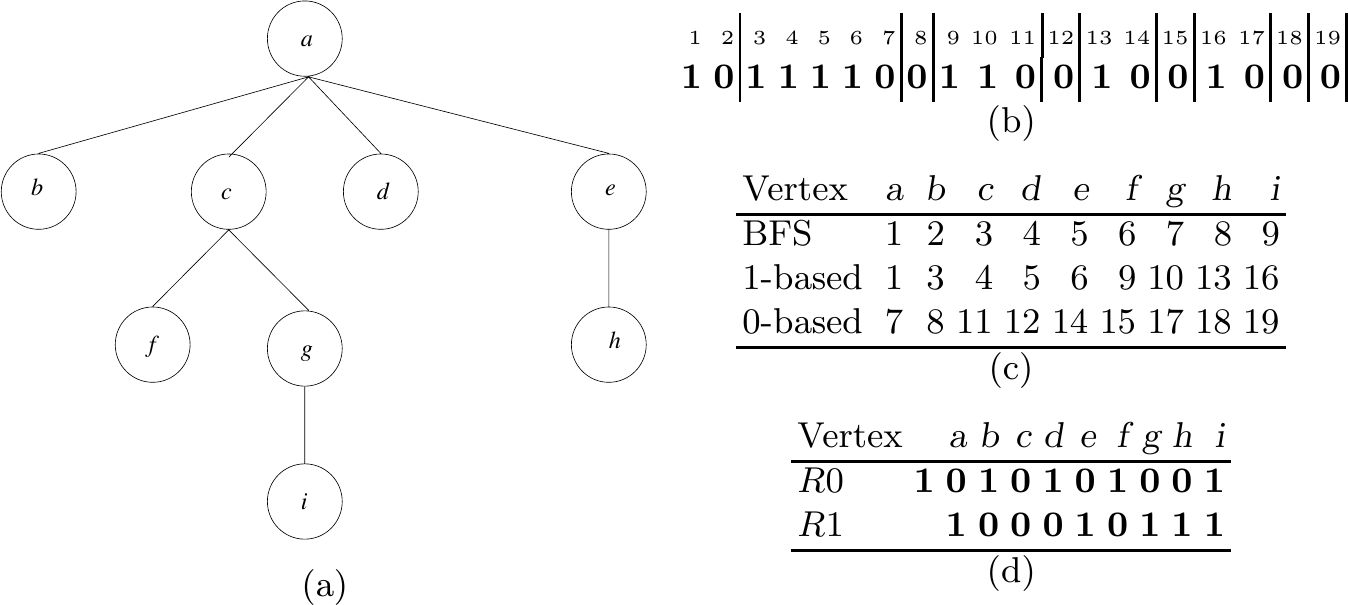
\includegraphics[width=0.8\textwidth]{LOUDS.jpg}
    \end{center}
    \begin{itemize}
        \item $R_0$: Nullfolgen (mit Längen $\ell_1,\ell_2\ldots\ell_z$) kombinieren zu $R_0=0^{\ell_1-1}10^{\ell_2-1}1\ldots0^{\ell_z-1}1$
        \item  $R_1$: Einsfolgen (mit Längen $\ell_1,\ell_2\ldots\ell_z$) kombinieren zu $R_1=0^{\ell_1-1}10^{\ell_2-1}1\ldots0^{\ell_z-1}1$
        \item Alle \texttt{select} Operationen auf LBS durchführbar durch \texttt{select}$_1$ und \texttt{rank}$_1$ auf $R_0$ oder $R_1$
        \item LOUDS++ nutzt $R_0$ und $R_1$
    \end{itemize}
\end{frame}

\begin{frame}{Ergebnisse}
    \begin{columns}
        \begin{column}{0.5\textwidth}
            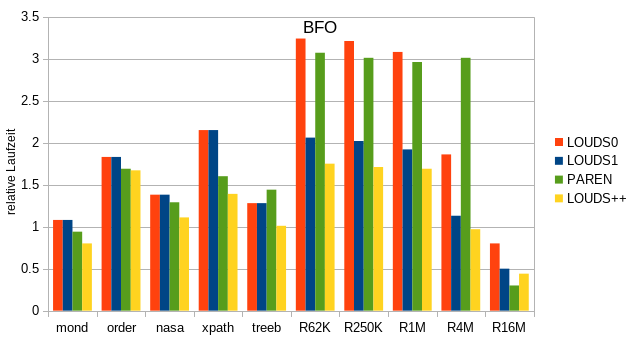
\includegraphics[width=1.08\textwidth]{graphics/BFO.png}
        \end{column}
        \begin{column}{0.5\textwidth}
            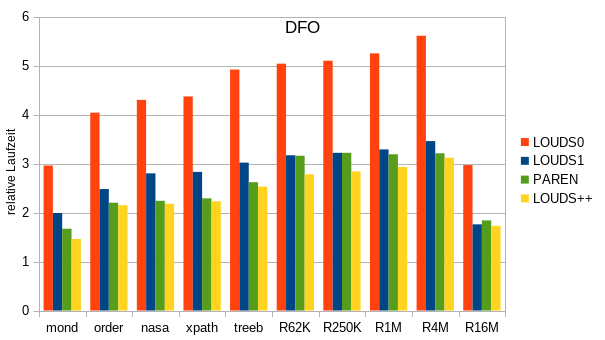
\includegraphics[width=1.03\textwidth]{graphics/DFO.png}
        \end{column}
    \end{columns}
\end{frame}

\end{document}